\ifx\wholebook\relax \else
% ------------------------

\documentclass{ctexart}
\usepackage[cn]{../../prelude}

\setcounter{page}{1}

\begin{document}

%--------------------------

% ================================================================
%                 COVER PAGE
% ================================================================

\title{从吃葡萄到世界杯,选择排序的进化}

\author{刘新宇
\thanks{{\bfseries 刘新宇 } \newline
  Email: liuxinyu95@gmail.com \newline}
  }

\maketitle
\fi

\markboth{选择排序}{初等算法}

\ifx\wholebook\relax
\chapter{从吃葡萄到世界杯,选择排序的进化}
\numberwithin{Exercise}{chapter}
\fi

\def\includetikz{}

% ================================================================
%                 Introduction
% ================================================================
\section{简介}
\label{introduction} \index{选择排序}

我们此前介绍了排序中的“hello world”―插入排序算法。本章中,我们介绍另外一种直观的排序方法―选择排序。最基本的选择排序在性能上不如分而治之的排序算法,如快速排序和归并排序。我们将会分析为什么选择排序的速度慢,并且从不同的角度改进它,最终进化到堆排序,从而达到基于比较的排序算法的性能上限$O(n \lg n)$。

选择排序的思想在日常生活中很常见。考虑一个小孩要吃掉一串葡萄。我们通常会发现两种类型的小孩,一种属于“乐观型”,每次吃掉最大的一颗;另一种属于“悲观型”,每次总吃掉最小的一颗。

第一种小孩实际上按照由大到小的顺序吃葡萄;第二种按照由小到大的顺序吃葡萄。实际上,孩子们把葡萄按照大小进行了\underline{排序},并且使用了选择排序的思想。
\begin{figure}[htbp]
  \centering
  \includegraphics[scale=0.6]{img/grapes-1.eps}
  \caption{总挑出最小的葡萄}
  \label{fig:eat-grapes}
\end{figure}

选择排序的算法可以描述如下。

为了将元素排序:

\begin{itemize}
\item 简单情况:如果序列为空,排序结果也为空;
\item 否则,我们找到最小的元素,将其附加到结果的后面。
\end{itemize}

注意上面描述的算法将元素按照升序排序;如果每次选择最大的元素,则排序结果是降序的。我们稍后会介绍如何将比较方法作为参数传入。

这一描述可以形式化为下面的公式。

\be
sort(A) =  \left \{
  \begin{array}
  {r@{\quad:\quad}l}
  \phi & A = \phi \\
  \{ m \} \cup sort(A') & otherwise
  \end{array}
\right.
\ee

其中$m$是序列$A$中的最小元素,$A'$是除$m$外的剩余元素。

\[
\begin{array}{l}
m = min(A) \\
A' = A - \{ m \}
\end{array}
\]

我们并不限定序列的具体数据结构。通常在命令式的环境中$A$是数组,在函数式环境中,$A$是单向链表。我们在后面将会看到,$A$甚至可以是其他数据结构。

这一算法也可以用命令式的方式给出:

\begin{algorithmic}[1]
\Function{Sort}{$A$}
  \State $X \gets \phi$
  \While{$A \neq \phi$}
    \State $x \gets$ \Call{Min}{$A$}
    \State $A \gets$ \Call{Del}{$A, x$}
    \State $X \gets$ \Call{Append}{$X, x$}
  \EndWhile
  \State \Return $X$
\EndFunction
\end{algorithmic}

图\ref{fig:sel-sort}描述了选择排序的过程。

\begin{figure}[htbp]
  \centering
  \includegraphics[scale=0.8]{img/sel-sort.ps}
  \caption{左侧部分为已排序的元素,算法不断从剩余部分选择最小元素附加的左侧的尾部}
  \label{fig:sel-sort}
\end{figure}

到目前为止,我们将“吃葡萄”的过程转换成了算法,但是没有考虑任何时间和空间上的开销。我们将结果保存在一个列表$X$中,把从剩余部分选择出的元素取出并添加到$X$的末尾。实际上,我们可以复用$A$中的空间实现原地排序。

具体方法是我们将最小的元素保存在$A$的第一个单元(cell)中(若$A$为数组,我们用单元来表示存储单位,若$A$为链表,我们用节点来表示存储单位),将第二小的元素保存在下一个单元中,接下来是第三个单元……

可以用交换的方法来实现这一排序策略。当我们找到第$i$小的元素后,我们将它和第$i$个位置的单元交换。

\begin{algorithmic}[1]
\Function{Sort}{$A$}
  \For{$i \gets 1$ to $|A|$}
    \State $m \gets$ \Call{Min}{$A[i...]$}
    \State \textproc{Exchange} $A[i] \leftrightarrow m$
  \EndFor
\EndFunction
\end{algorithmic}

记$A = \{a_1, a_2, ..., a_n\}$,任何时候,当我们处理第$i$个元素时,所有在$i$之前的部分$\{a_1, a_2, ..., a_{i-1}\}$都已经排好序了。我们找到$\{a_i, a_{i+1}, ..., a_n\}$中的最小元素,然后将其和$a_i$交换,这样第$i$个位置就保存了正确的元素。重复这一过程直到最后一个元素。

图\ref{fig:in-place-ssort}描述了这一思路。

\begin{figure}[htbp]
  \centering
  \begin{tikzpicture}[scale=0.8]
    \draw (0, 0) rectangle (3.5,1) node[pos=.5] {...已序元素...};
    \draw (4, 0) rectangle (5, 1) node (x) [pos=.5] {$x$};
    \draw (5, 0) rectangle (6, 1) node[pos=.5] {...};
    \draw (6, 0) rectangle (7, 1) node (min) [pos=.5] {$min$};
    \draw (7, 0) rectangle (8, 1) node[pos=.5] {...};
    \draw[thick, <->] (x) edge[bend left=45] node [above] {交换} (min);
  \end{tikzpicture}
  \caption{左侧部分为已序元素,不断从剩余元素中找到最小的存储到正确的位置}
  \label{fig:in-place-ssort}
\end{figure}

% ================================================================
% Find the minimum
% ================================================================
\section{查找最小元素}
\index{选择排序!查找最小元素}

我们尚未完全实现选择排序,如何查找最小(或最大)的元素仍然是一个黑盒子。小孩子们是如何找到最小或最大的一粒葡萄的?这对于计算机算法来说也是一个有趣的题目。

虽然不够快,但是最简单的方法是对所有的元素进行一次扫描。存在几种不同的方法来实现扫描的过程。假设要选出最大的一粒葡萄。我们任选一颗,将它和另外一颗比较,然后留下较大的;此后我们再选另外一颗,和手里留下的这颗比较,并留下最大的。重复这一“选取―比较”的过程直到比较完所有的葡萄。

实践一下,我们会发现,如果不对比较过的葡萄做记号,很快就会搞乱,我们会忘记哪些葡萄比较过了,哪些还没有。有两种方法可以解决这一问题,它们分别适合不同的数据结构。

\subsection{标记}
第一种方法是将葡萄标记上编号,例如:$\{1, 2, ..., n\}$,然后按照编号的顺序进行比较。先比较第一号葡萄和第二号葡萄,选择较大的留下;然后用第三号葡萄做比较……重复这一步骤直到第$n$号葡萄。标记方法很适合处理数组。

\begin{algorithmic}[1]
\Function{Min}{$A$}
  \State $m \gets A[1]$
  \For{$i \gets 2$ to $|A|$}
    \If{$A[i] < m$}
      \State $m \gets A[i]$
    \EndIf
  \EndFor
  \State \Return $m$
\EndFunction
\end{algorithmic}

使用\textproc{Min}函数,我们可以最终完成基本的选择排序(没有任何空间和时间上的优化)。

上述查找最小元素的方法返回的是元素的值而非它的位置(葡萄的编号),如果要实现原地排序,还需要做一些调整。某些语言,如C++支持返回引用作为结果,因此可以直接实现元素的交换。

\lstset{language=C++}
\begin{lstlisting}
template<typename T>
T& min(T* from, T* to) {
    T* m;
    for (m = from++; from != to; ++from)
        if (*from < *m)
            m = from;
    return *m;
}

template<typename T>
void ssort(T* xs, int n) {
    for (int i = 0; i < n; ++i)
        std::swap(xs[i], min(xs+i, xs+n));
}
\end{lstlisting}

在不支持引用语意的环境中,可以返回元素的位置,而不是值作为结果。

\begin{algorithmic}[1]
\Function{Min-At}{$A$}
  \State $m \gets$ \Call{First-Index}{$A$}
  \For{$i \gets m + 1 $ to $|A|$}
    \If{$A[i] < A[m]$}
      \State $m \gets i$
    \EndIf
  \EndFor
  \State \Return $m$
\EndFunction
\end{algorithmic}

传入\textproc{Min-At}的数组实际是$A$的片断$A[i...]$,我们假设第一个元素$A[i]$是最小的一个,并且逐一检查元素$A[i+1], A[i+2], ...$。函数\textproc{First-Index}()用于从参数中获取索引$i$。

下面的Python例子程序,根据这一思路实现了基本的原地选择排序算法。它直接将数组片断的信息传入,并使用最小元素的位置。

\lstset{language=Python}
\begin{lstlisting}
def ssort(xs):
    n = len(xs)
    for i in range(n):
        m = min_at(xs, i, n)
        (xs[i], xs[m]) = (xs[m], xs[i])
    return xs

def min_at(xs, i, n):
    m = i;
    for j in range(i+1, n):
        if xs[j] < xs[m]:
            m = j
    return m
\end{lstlisting}

\subsection{分组}
\index{选择排序!尾递归查找最小值}

另外一种方法是将全部葡萄分成两部分:一组包含已经检查并比较过的所有葡萄,另外一组包含剩余未比较过的。记这两组葡萄为$A$和$B$、全部的元素(葡萄)为$L$。在开始的时候,我们尚未处理任何葡萄,因此$A$为空($\phi$),$B$包含全部葡萄。我们可以从$B$中任选两颗葡萄进行比较,然后将较小的一颗放入$A$。此后我们不断从$B$中选择葡萄,和上次比较的获胜者(较大的一颗)对比直到$B$变成空。这时,最后的获胜者就是最小的元素,而$A$中包含$L - \{min(L)\}$,可以用于下一轮的最小值查找。

这一方法的不变关系(invariant)为:在任何时候我们有:$L = A \cup \{m\} \cup B$,其中$m$为目前找到的获胜者。

这一方法无需对葡萄进行编号。它适用于任何可被遍历的数据结构,包括链表等。令$b_1$为非空序列$B$中的任一元素,$B'$为除$b_1$外的剩余元素,上述方法可以形式化为如下函数。

\be
min'(A, m, B) =  \left \{
  \begin{array}
  {r@{\quad:\quad}l}
  (m, A) & B = \phi \\
  min'(A \cup \{m\}, b_1, B') & b_1 < m \\
  min'(A \cup \{b_1\}, m, B') & otherwise
  \end{array}
\right.
\ee

为了选出最小元素,我们调用这一函数并传入空序列$A$。选取任何元素(例如第一个)来初始化$m$:

\be
extractMin(L) = min'(\phi, l_1, L')
\ee

其中$L'$包含$L$中除$l_1$以外的剩余元素。算法$extractMin$不仅查找最小元素,还返回剩余元素以用于接下来的排序。下面的Haskell例子程序实现了这一算法。

\lstset{language=Haskell}
\begin{lstlisting}[style=Haskell]
sort [] = []
sort xs = x : sort xs' where
  (x, xs') = extractMin xs

extractMin (x:xs) = min' [] x xs where
  min' ys m [] = (m, ys)
  min' ys m (x:xs) = if m < x then min' (x:ys) m xs else min' (m:ys) x xs
\end{lstlisting}

第一行处理边界情况,空序列的排序结果仍为空;第二行确保序列中至少含有一个元素,因此\texttt{extractMin}函数无需再做额外的模式匹配。

有读者认为函数\texttt{min'}第二个子式应该实现如下:

\begin{lstlisting}[style=Haskell]
min' ys m (x:xs) = if m < x then min' ys ++ [x] m xs
                            else min' ys ++ [m] x xs
\end{lstlisting}

否则函数会返回逆序的列表。但这里我们需要用“cons”\footnote{cons来自Lisp语言,表示将一个元素附加到一个链表的头部。详见附录A。}而不是追加。因为追加操作的复杂度是线性的,和序列$A$的长度成正比,而“cons”是常数时间$O(1)$的。我们并不需要保持待排序元素的顺序,因为排序过程本身就是对顺序的一种改变。

当然,既保持元素的相对顺序\footnote{称为稳定排序(stable sort)},又能高效地查找最小元素,而不退化成平方复杂度是可以实现的。下面的定义满足了这一限制:

\be
extractMin(L) = \left \{
  \begin{array}
  {r@{\quad:\quad}l}
  (l_1, \phi) & |L| = 1 \\
  (l_1, L') & l_1 < m, (m, L'') = extractMin(L') \\
  (m, {l_1} \cup L'') & otherwise
  \end{array}
\right.
\ee

如果$L$只含有一个元素(称为singleton),最小值就是这唯一的元素。否则记$l_1$为$L$中的第一个元素,除$l_1$以外的剩余元素为$L'$,即$L' = \{ l_2, l_3, ...\}$。算法递归地从$L'$中查找最小元素,结果记为$(m, L'')$,其中$m$是$L'$中的最小元素,而$L''$包含除$m$外的剩余元素。比较$l_1$和$m$以决定哪个是最终的最小值。

下面的Haskell程序实现了这一版本的选择排序。

\begin{lstlisting}[style=Haskell]
sort [] = []
sort xs = x : sort xs' where
  (x, xs') = extractMin xs

extractMin [x] = (x, [])
extractMin (x:xs) = if x < m then (x, xs) else (m, x:xs') where
  (m, xs') = extractMin xs
\end{lstlisting}

这里仅仅使用了“cons”操作,而无需“追加”操作。因为算法从右向左处理列表。但是这会有一些额外开销,程序通常需要使用堆栈来保存递归的环境。元素间的相对顺序通过递归来加以保证。读者可以参考附录中关于“尾递归”的内容。

\subsection{选择排序的性能}

无论是标记法,还是分组法都需要在每轮中检查所有未排好的元素以挑选出最小值;总共进行了$n$次挑选。因此处理时间为:$n + (n-1) + (n-2) + ... + 1$次比较,即$\frac{n(n+1)}{2}$。选择排序是平方时间$O(n^2)$的算法。

和此前介绍的插入排序相比,选择排序在最好、最差和平均情况下的性能是相同的,而插入排序在最好情况下性能为线性时间$O(n)$(元素存储在一个链表中,并且顺序为逆序),最差情况下性能为平方时间$O(n^2)$。

在接下来的部分,我们将分析为何选择排序的性能较差,并尝试逐步改进它。

\begin{Exercise}

\begin{itemize}
\item 选择一门编程语言实现基本的命令式选择排序(非原地排序版本)。和原地排序的算法进行对比,分析时间和空间上的效率。
\end{itemize}

\end{Exercise}

% ================================================================
% Improvement 1
% ================================================================

\section{细微改进}

本节介绍针对选择排序的一些细微改进,首先我们通过参数化,将排序算法变得通用;然后对算法结构进行一些细微调整,使得它更为紧凑。最后我们介绍“鸡尾酒排序”将循环次数减半。

\subsection{比较方法参数化}
\index{选择排序!比较方法参数化}

在改进性能前,我们先将前面给出的选择排序算法变得更加通用,以便能处理各种排序条件。

我们可以看到存在两种完全相反的排序需要:升序排序和降序排序。对于前者,需要不断查找最小元素;而对于后者,需要不断寻找最大元素。实际应用中,远非这两种情况,还存在各种各样的排序标准,例如按照尺寸、重量、年龄……进行排序。

我们可以将具体的排序标准作为一个比较函数传入选择排序算法,如下:

\be
sort(c, L) = \left \{
  \begin{array}
  {r@{\quad:\quad}l}
  \phi & L = \phi \\
  {m} \cup sort(c, L'') & L \neq \phi, (m, L'') = extract(c, L')
  \end{array}
\right.
\ee

其中$extract(c, L)$的定义为:

\be
extract(c, L) = \left \{
  \begin{array}
  {r@{\quad:\quad}l}
  (l_1, \phi) & |L| = 1 \\
  (l_1, L') & c(l_1, m), (m, L'') = extract(c, L') \\
  (m, \{l_1\} \cup L'') & \lnot c(l_1, m)
  \end{array}
\right.
\ee

这里$c$是一个比较函数,它接受两个元素,将它们相比并决定哪个的顺序在前面。将“小于”操作$(<)$传入,就是我们此前给出的选择排序实现。

有些环境需要传入全序(total ordering)的比较函数,也就是说比较结果为“小于”、“等于”或者“大于”中的一个。对于选择排序,并不需要这样强的限制,$c$只要检查“小于”是否满足即可。但是作为最低要求,比较函数必须满足严格弱序(strict weak ordering)\cite{wiki-sweak-order}:

\begin{itemize}
\item 非自反性(Irreflexivity),对于任何$x$,$x < x$不成立;
\item 非对称性(Asymmetric),对任何$x$和$y$,若$x < y$成立,则$y < x$不成立;
\item 传递性(Transitivity), 对任何$x$、$y$和$z$,若$x < y$且$y < z$,则$x < z$成立。
\end{itemize}

下面的Scheme/Lisp例子程序实现了参数化的选择排序。Scheme/Lisp的词法作用域(lexical scope)可以简化比较函数的传递。

\lstset{language=Lisp}
\begin{lstlisting}
(define (sel-sort-by ltp? lst)
  (define (ssort lst)
    (if (null? lst)
        lst
        (let ((p (extract-min lst)))
          (cons (car p) (ssort (cdr p))))))
  (define (extract-min lst)
    (if (null? (cdr lst))
        lst
        (let ((p (extract-min (cdr lst))))
          (if (ltp? (car lst) (car p))
              lst
              (cons (car p) (cons (car lst) (cdr p)))))))
  (ssort lst))
\end{lstlisting}

其中\texttt{ssort}和\texttt{extract-min}都是内部函数,它们都可以直接使用比较函数\texttt{ltp?}。将$<$传入就可以得到普通的升序排序结果。

\lstset{language=Lisp}
\begin{lstlisting}
(sel-sort-by < '(3 1 2 4 5 10 9))
;Value 16: (1 2 3 4 5 9 10)
\end{lstlisting}

在命令式实现中也可以将比较函数参数化,我们将其作为练习留给读者。

简单起见,本章的后继部分我们仅仅考虑元素的升序排序,除非必要,我们不将比较函数作为参数传入。

\subsection{细微调整}

基本的命令式原地选择排序算法遍历了所有的元素,每次查找出最小的。我们可以把最小值的查找直接实现为一个内重循环,从而使程序变得更加紧凑。

\begin{algorithmic}[1]
\Procedure{Sort}{$A$}
  \For{ $i \gets 1$ to $|A|$}
    \State $m \gets i$
    \For{$j \gets i+1$ to $|A|$}
      \If{$A[i] < A[m]$}
        \State $m \gets i$
      \EndIf
    \EndFor
    \State \textproc{Exchange} $A[i] \leftrightarrow A[m]$
  \EndFor
\EndProcedure
\end{algorithmic}

进一步观察,我们需要将$n$个元素排序,当前$n-1$个元素排好后,最后剩下的一个元素,必然是第$n$大的。因此无需再进行一次最小值查找。这样外重循环的次数可以减少一次变成$n-1$。

还有一处可以进行细微调整,如果第$i$大的元素恰好是$A[i]$,我们无需进行交换操作。最终实现可以调整为:

\begin{algorithmic}[1]
\Procedure{Sort}{$A$}
  \For{ $i \gets 1$ to $|A|-1$}
    \State $m \gets i$
    \For{$j \gets i+1$ to $|A|$}
      \If{$A[i] < A[m]$}
        \State $m \gets i$
      \EndIf
    \EndFor
    \If{$m \neq i$}
      \State \textproc{Exchange} $A[i] \leftrightarrow A[m]$
    \EndIf
  \EndFor
\EndProcedure
\end{algorithmic}

显然,上面这些调整都对整体的复杂度没有影响。

\subsection{鸡尾酒排序(Cock-tail sort)}
\index{鸡尾酒排序}

Knuth给出过一个另一种选择排序的实现\cite{TAOCP}。每次不是查找最小元素,而是最大元素,将其放在末尾位置。如下:

\begin{algorithmic}[1]
\Procedure{Sort'}{$A$}
  \For{ $i \gets |A|$ down-to $2$}
    \State $m \gets i$
    \For{$j \gets 1$ to $i-1$}
      \If{$A[m] < A[i]$}
        \State $m \gets i$
      \EndIf
    \EndFor
    \State \textproc{Exchange} $A[i] \leftrightarrow A[m]$
  \EndFor
\EndProcedure
\end{algorithmic}

如图\ref{fig:knuth-ssort}所示,任何时候,最右侧的元素都是已序的。算法扫描未排序元素,定位到其中的最大值,然后交换到未排序部分的末尾。

\begin{figure}[htbp]
  \centering
  \begin{tikzpicture}[scale=0.8]
    \draw (5, 0) rectangle (6, 1) node[pos=.5] {...};
    \draw (6, 0) rectangle (7, 1) node (max) [pos=.5] {$max$};
    \draw (7, 0) rectangle (8, 1) node[pos=.5] {...};
    \draw (8, 0) rectangle (9, 1) node (x) [pos=.5] {$x$};
    \draw (10,0) rectangle (13.5,1) node[pos=.5] {...已序元素...};
    \draw[thick, <->] (x) edge[bend right=45] node [above] {交换} (max);
  \end{tikzpicture}
  \caption{每次选择最大的元素放到末尾}
  \label{fig:knuth-ssort}
\end{figure}

这一版本的实现说明,每次选择最大的元素也可以实现升序排序。进一步说,我们每次扫描可以同时查找最小值和最大值,分别将最小值放到开头,将最大值放到末尾。这样可以将排序性能略微提高(外重循环次数减半)。我们称这一算法为“鸡尾酒排序”。

\begin{algorithmic}[1]
\Procedure{Sort}{$A$}
  \For{$i \gets 1 $ to $\lfloor \frac{|A|}{2} \rfloor$}
    \State $min \gets i$
    \State $max \gets |A| + 1 - i$
    \If{$A[max] < A[min]$}
      \State \textproc{Exchange} $A[min] \leftrightarrow A[max]$
    \EndIf
    \For{$j \gets i + 1$ to $|A| - i$}
      \If{$A[j] < A[min]$}
        \State $min \gets j$
      \EndIf
      \If{$A[max] < A[j]$}
        \State $max \gets j$
      \EndIf
    \EndFor
    \State \textproc{Exchange} $A[i] \leftrightarrow A[min]$
    \State \textproc{Exchange} $A[|A|+1-i] \leftrightarrow A[max]$
  \EndFor
\EndProcedure
\end{algorithmic}

图\ref{fig:cock-tail-sort}描述了这一算法,任何时候,左侧部分和右侧部分都包含了已序元素。较小的在左侧,较大的在右侧。算法扫描未排序的部分,定位到最小和最大的两个元素,然后分别将它们交换到未排序部分的开头和末尾。

\begin{figure}[htbp]
  \centering
  \begin{tikzpicture}[scale=0.8]
    \draw (0,0) rectangle (3.5,1) node[pos=.5] {...已序较小元素...};
    \draw (4, 0) rectangle (5, 1) node (x) [pos=.5] {$x$};
    \draw (5, 0) rectangle (6, 1) node[pos=.5] {...};
    \draw (6, 0) rectangle (7, 1) node (max) [pos=.5] {$max$};
    \draw (7, 0) rectangle (8, 1) node[pos=.5] {...};
    \draw (8, 0) rectangle (9, 1) node (min) [pos=.5] {$min$};
    \draw (9, 0) rectangle (10, 1) node[pos=.5] {...};
    \draw (10, 0) rectangle (11, 1) node (y) [pos=.5] {$y$};
    \draw (12,0) rectangle (15.5,1) node[pos=.5] {...已序较大元素...};
    \draw[thick, <->] (x) edge[bend right=45] node [below] {交换} (min);
    \draw[thick, <->] (y) edge[bend right=45] node [above] {交换} (max);
  \end{tikzpicture}
  \caption{一次扫描同时定位出最小和最大元素,然后将它们放到正确的位置}
  \label{fig:cock-tail-sort}
\end{figure}


注意,在内重循环开始前,如果最右侧的元素小于最左侧的元素,需要将它们交换。这是因为我们的扫描范围不包括两端上的元素。另外一种方法是,在内重循环扫描前,我们将最小和最大元素同时初始化为第一个未排序元素。但是这会产生一个新问题:由于我们在内重循环扫描后要做两次交换操作,有可能第一次交换会改变我们刚刚找到的最大元素或最小元素的位置,这样第二次交换就会产生不正确的结果。我们把如何解决这一问题留给读者作为练习。

下面的Python例子程序实现了鸡尾酒排序。

\lstset{language=Python}
\begin{lstlisting}
def cocktail_sort(xs):
    n = len(xs)
    for i in range(n / 2):
        (mi, ma) = (i, n - 1 -i)
        if xs[ma] < xs[mi]:
            (xs[mi], xs[ma]) = (xs[ma], xs[mi])
        for j in range(i+1, n - 1 - i):
            if xs[j] < xs[mi]:
                mi = j
            if xs[ma] < xs[j]:
                ma = j
        (xs[i], xs[mi]) = (xs[mi], xs[i])
        (xs[n - 1 - i], xs[ma]) = (xs[ma], xs[n - 1 - i])
    return xs
\end{lstlisting}

鸡尾酒排序也可以用函数式的方式加以实现。一个直观的描述为:

\begin{itemize}
  \item 边界情况:若待排序的序列为空或者仅含有一个元素,则排序结果为原序列;
  \item 否则,找到最小和最大值,分别放到开头和结尾位置,然后递归地将剩余元素排序。
\end{itemize}

算法可以形式化为如下函数。

\be
sort(L) = \left \{
  \begin{array}
  {r@{\quad:\quad}l}
  L & |L| \leq 1 \\
  \{ l_{min} \} \cup sort(L'') \cup \{ l_{max} \} & otherwise
  \end{array}
\right.
\ee

其中,函数$select(L)$从序列$L$中抽取出最小值和最大值。

\[
(l_{min}, L'', l_{max}) = select(L)
\]

注意,最小值实际被直接链结到递归排序结果的前面。语意上是一个常数时间$O(1)$的“cons”操作(参考本书附录A)。但是最大值被追加到末尾,这一操作的代价较大,通常需要线性时间$O(n)$。我们稍后再优化它。

函数$select(L)$扫描传入的序列查找最小值和最大值,它的定义为:

\be
select(L) =  \left \{
  \begin{array}
  {r@{\quad:\quad}l}
  (min(l_1, l_2), max(l_1, l_2)) & L = \{ l_1, l_2\} \\
  (l_1, \{ l_{min}\} \cup L'', l_{max}) & l_1 < l_{min} \\
  (l_{min}, \{l_{max}\} \cup L'', l_1) & l_{max} < l_1 \\
  (l_{min}, \{l_1\} \cup L'', l_{max}) & otherwise
  \end{array}
\right.
\ee

其中$(l_{min}, L'', l_{max}) = select(L')$,$L'$是除去$l_1$外的剩余元素。如果序列中仅有两个元素,我们选择较小的最为最小值,较大的作为最大值。剩余序列为空。这是边界情况。否则,我们取出第一个元素$l_1$,然后递归地在剩余元素中抽取最小和最大值并和$l_1$做比较以决定最终的结果。

注意所有情况下,我们都不需要做结果列表的追加操作。但是抽取过程需要扫描全部元素,因此性能是线性时间$O(n)$的。

下面的Haskell例子程序实现了这一算法。

\lstset{language=Haskell}
\begin{lstlisting}[style=Haskell]
csort [] = []
csort [x] = [x]
csort xs = mi : csort xs' ++ [ma] where
  (mi, xs', ma) = extractMinMax xs

extractMinMax [x, y] = (min x y, [], max x y)
extractMinMax (x:xs) | x < mi = (x, mi:xs', ma)
                     | ma < x = (mi, ma:xs', x)
                     | otherwise = (mi, x:xs', ma)
  where (mi, xs', ma) = extractMinMax xs
\end{lstlisting}

此前我们指出追加操作的性能开销较大。这一问题可以分两步解决。第一步是将鸡尾酒排序转换为尾递归。左侧包含较小的已序元素,记这一部分为$A$;右侧包含较大的已序元素,记这一部分为$B$。如图\ref{fig:cock-tail-sort}所示。我们用$A$和$B$作为累积器(accumulator),鸡尾酒排序的尾递归实现如下:

\be
sort'(A, L, B) = \left \{
  \begin{array}
  {r@{\quad:\quad}l}
  A \cup L \cup B & L = \phi \lor |L| = 1 \\
  sort'(A \cup \{ l_{min}\}, L'', \{ l_{max}\} \cup B) & otherwise
  \end{array}
\right.
\ee

其中$l_{min}$、$l_{max}$和$L''$的定义同上。排序开始时,我们传入空的$A$和$B$:

\[
sort(L) = sort'(\phi, L, \phi)
\]

先跳过边界情况,注意到追加操作仅仅发生在$A \cup \{l_{min} \}$;而$l_{max}$则直接被链结到$B$的前面。每次递归调用都会产生一次追加操作。为了消除它,我们可以将$A$保存为逆序$\overleftarrow{A}$,这样就可以将$l_{min}$链结到前面而不是执行一次耗时的追加。记$cons(x, L) = \{x\} \cup L$,$append(L, x) = L \cup \{x\}$,我们有如下等式:

\be
\begin{array}{rl}
append(L, x) & = reverse(cons(x, reverse(L))) \\
             & = reverse(cons(x, \overleftarrow{L}))
\end{array}
\ee

最后,我们执行一次反转操作将$\overleftarrow{A}$转换回$A$。根据这一思路,算法可进一步被改进如下:

\be
sort'(A, L, B) = \left \{
  \begin{array}
  {r@{\quad:\quad}l}
  reverse(A) \cup B & L = \phi \\
  reverse(\{l_1\} \cup A) \cup B & |L| = 1 \\
  sort'(\{l_{min}\} \cup A, L'', \{l_{max}\} \cup B)
  \end{array}
\right.
\ee

下面的Haskell例子程序实现了这一改进。

\lstset{language=Haskell}
\begin{lstlisting}[style=Haskell]
csort' xs = cocktail [] xs [] where
  cocktail as [] bs = reverse as ++ bs
  cocktail as [x] bs = reverse (x:as) ++ bs
  cocktail as xs bs = let (mi, xs', ma) = extractMinMax xs
                      in cocktail (mi:as) xs' (ma:bs)
\end{lstlisting}

\begin{Exercise}
  \begin{itemize}
    \item 用动态语言和静态语言分别实现基本的选择排序算法,将比较函数用参数传入。在静态语言中,如何声明比较函数的类型才能做到更加通用(generic)?
   \item 使用一门编程语言实现Knuth给出的选择排序。
   \item 另一种实现鸡尾酒排序的方法是在内重循环前,假定第$i$个元素既是最小值,也是最大值。内重循环结束后,最小值和最大值被定位出来,需要将最小值交换到第$i$个位置,将最大值交换到第$|A|+1-i$个位置。请用一门命令式语言实现这一解法。注意以下特殊的边界情况:
    \begin{itemize}
      \item $A = \{max, min, ...\}$;
      \item $A = \{..., max, min\}$;
      \item $A = \{max, ..., min\}$.
    \end{itemize}
  \item 使用fold来实现$select(L)$函数。
  \end{itemize}
\end{Exercise}

% ================================================================
% Improvement 2
% ================================================================

\section{本质改进}

虽然鸡尾酒排序将循环次数减半,但是性能仍然是平方级的。如果序列很大,和其他分而治之的排序相比,选择排序的性能明显落后。

为了从本质上改进选择排序,我们必须分析瓶颈出现在哪里。为了通过比较大小进行排序,必须检查所有元素间的大小顺序。因此外重循环是必须的。但是为了选出最小元素,我们必须每次都扫描全部元素么?当查找第一个最小元素时,我们实际遍历了全部的序列,因此我们知道哪些元素相对较小,哪些元素相对较大。

问题在于当查找后继的最小元素时,我们没有复用这些已经获取到的关于相对大小的信息。而是从零开始再次进行遍历。

提高选择排序的关键点在于重用已有的结果。存在几种不同的方法,其中一种是从足球比赛中得到启发的。

\subsection{锦标赛淘汰法}
\index{锦标赛淘汰法}

足球世界杯每四年举办一次。来自各个大洲的32支球队最终进入决赛。1982年前,决赛阶段只有16支球队\cite{wiki-wc}。

简单起见,让我们回到1978年,并且想像一种特殊的方法来决定谁是冠军:在第一轮比赛中,所有参赛球队被分为8组进行比赛;比赛产生8支获胜球队,其余8支被淘汰。接下来,在第二轮比赛中,8支球队被分成4组。比赛产生4支获胜球队;然后这4支球队分成两对,比赛产生最终的两支球队争夺冠军。

经过4轮比赛,冠军就可产生。总共的比赛场次为:$8+4+2+1 = 15$。但是我们并不满足仅仅知道谁是冠军,我们还想知道哪支球队是亚军。

有人会问最后一场比赛中被冠军击败的队伍不是亚军么?在真实的世界杯中,的确如此。但是这个规则在某种程度上并不公平。

我们常常听说过“死亡之组”,假设巴西队一开始就和荷兰队进行比赛。虽然它们两个都是强队,但是必须有一支在一上来就被淘汰。这支被淘汰的球队,很可能会打败除冠军外的其他所有球队。图\ref{fig:tournament-tree-1}描述了这一情况。

\begin{figure}[htbp]
  \centering
  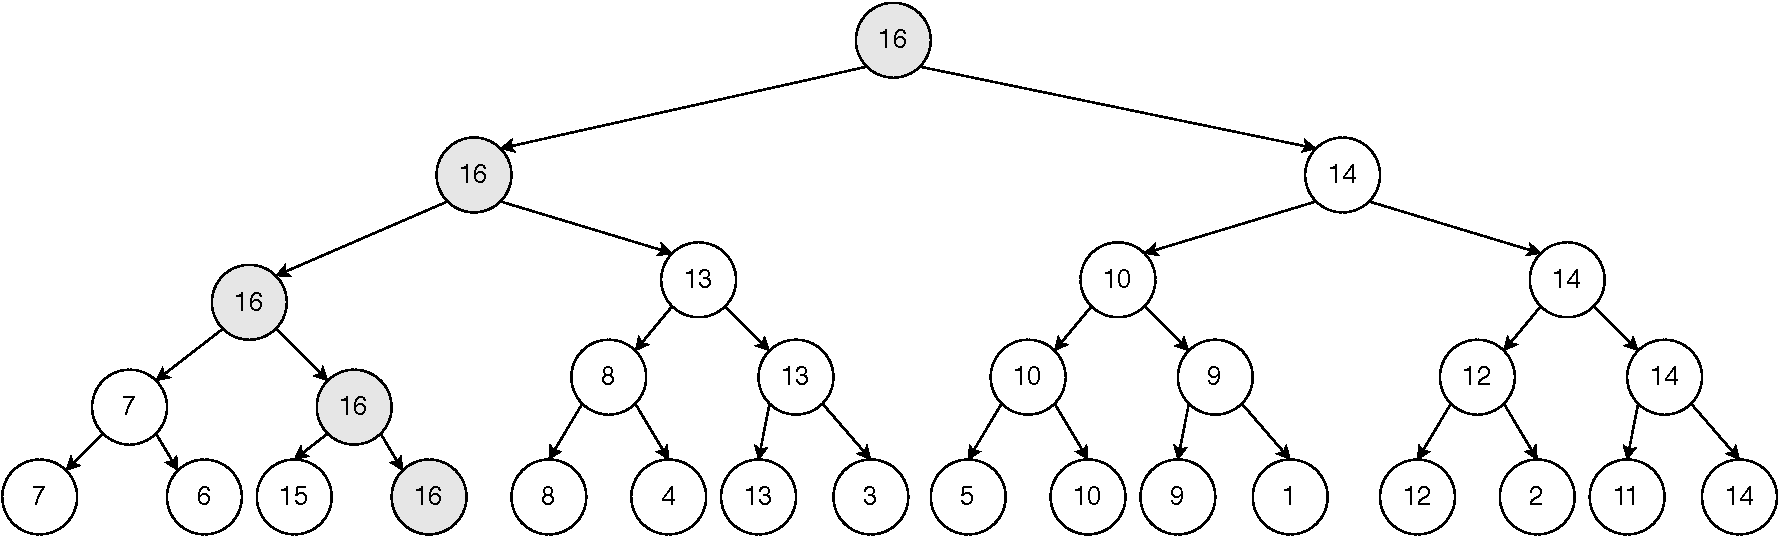
\includegraphics[scale=0.6]{img/tournament-tree-1.ps}
  \caption{元素15在第一轮就被淘汰}
  \label{fig:tournament-tree-1}
\end{figure}

假设每支队伍有一个代表其实力的数字。数字越大,实力越强。假设数字较大的队永远会战胜数字较小的队。虽然现实中不会这样,但是我们可以由此简化模型,给出一个锦标赛淘汰法的实现。代表冠军的数字为16,根据假设的规则,数字14不是亚军,而是在第一轮就被淘汰的15.

我们需要找到一种快速的方法在锦标赛树中找到第二个最大值。此后,我们只要不断重复这一方法,逐一找出第三大,第四大……就可以完成基于选择的排序。

一种办法是,把冠军的数字变成一个很小的值(例如$-\infty$),这样以后它就不会被选中,这样第二名就会成为新的冠军。假设有$2^m$支球队,其中$m$是某个自然数,仍然需要$2^{m-1} + 2^{m-2} + ... + 2 + 1 = 2^m-1$次比较才能产生新的冠军,这和第一次寻找冠军花费的代价相同。

实际上,我们无需再进行自底向上的比较。锦标赛树中保存了足够的顺序信息。实力第二强的队,一定在某个时刻被冠军击败,否则它就会是最终的冠军。因此我们可以从锦标赛树的根节点出发,沿着产生冠军的路径向叶子方向遍历,在这条路径上寻找第二强的队。

图\ref{fig:tournament-tree-1}中,这条路径被标记为灰色,需要检查的元素包括$\{14, 13, 7, 15\}$,根据这一思想,我们将算法调整如下:

\begin{enumerate}
\item 从待排序元素构建一棵锦标赛树,冠军(最大值)位于树根;
\item 取出树根,自顶向下沿着冠军路径将最大值替换为$-\infty$;
\item 自底向上沿着刚才的路径回溯,找出新的冠军,并将其置于树根;
\item 重复步骤2,直到所有的元素都被取出。
\end{enumerate}

图\ref{fig:tournament-tree-4}给出了这一排序的前几个步骤。

\captionsetup[subfigure]{labelformat=empty, margin=10pt}
\begin{figure}[htbp]
  \centering
  \subcaptionbox{取出16,将其替换为$-\infty$,15上升为新的根}{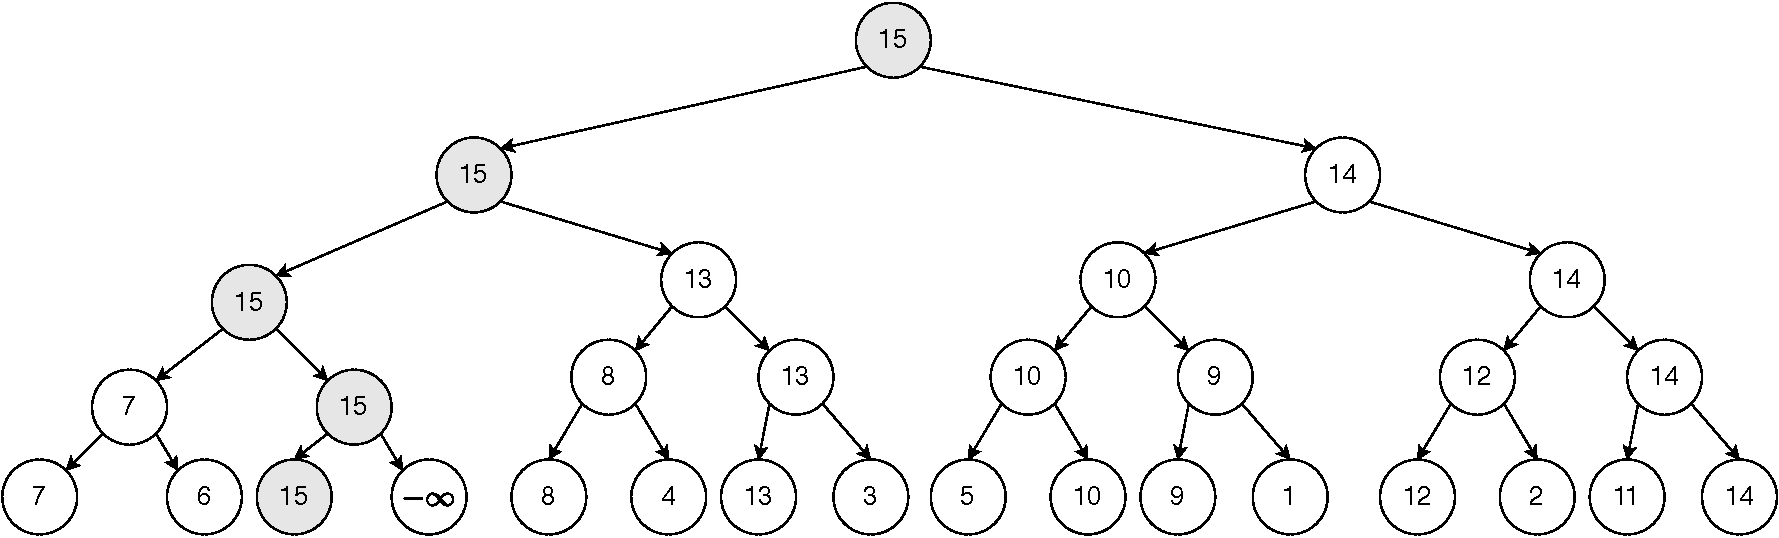
\includegraphics[scale=0.6]{img/tournament-tree-2.ps}} \\
  \subcaptionbox{取出15,将其替换为$-\infty$,14上升为新的根}{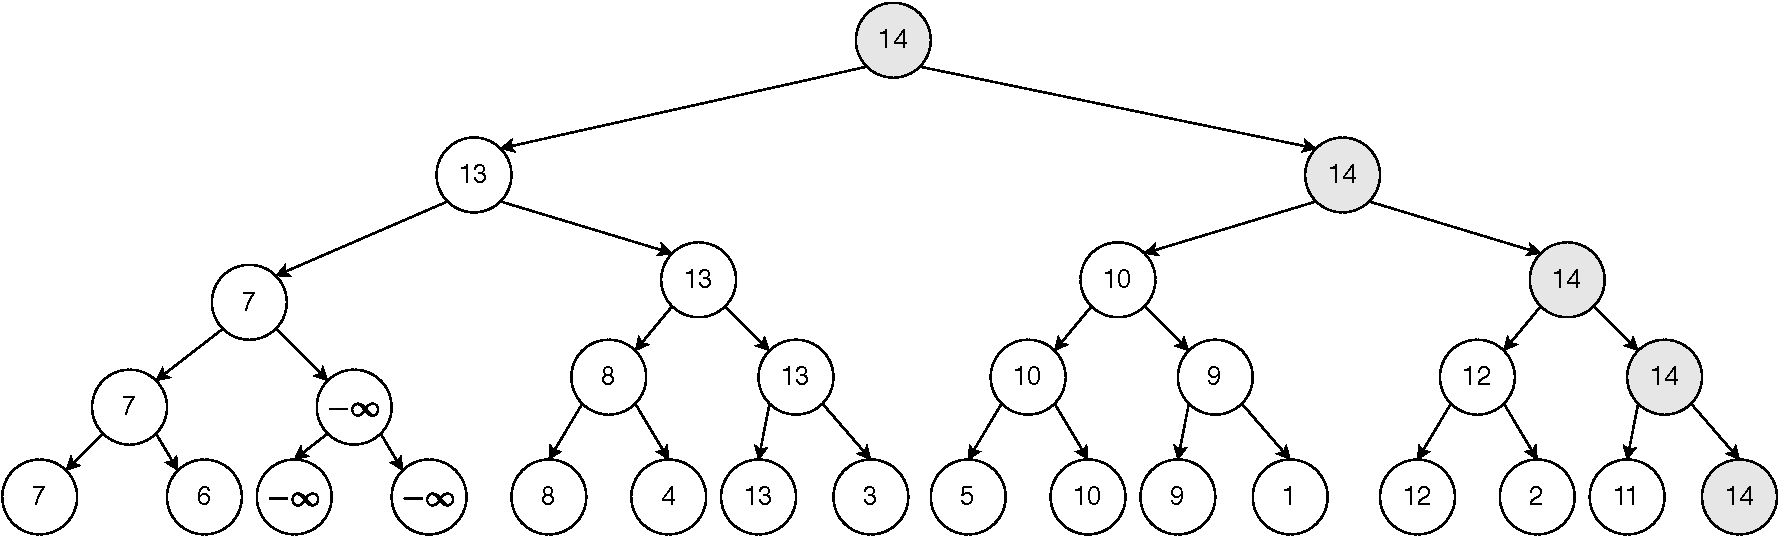
\includegraphics[scale=0.6]{img/tournament-tree-3.ps}} \\
  \subcaptionbox{取出14,将其替换为$-\infty$,13上升为新的根}{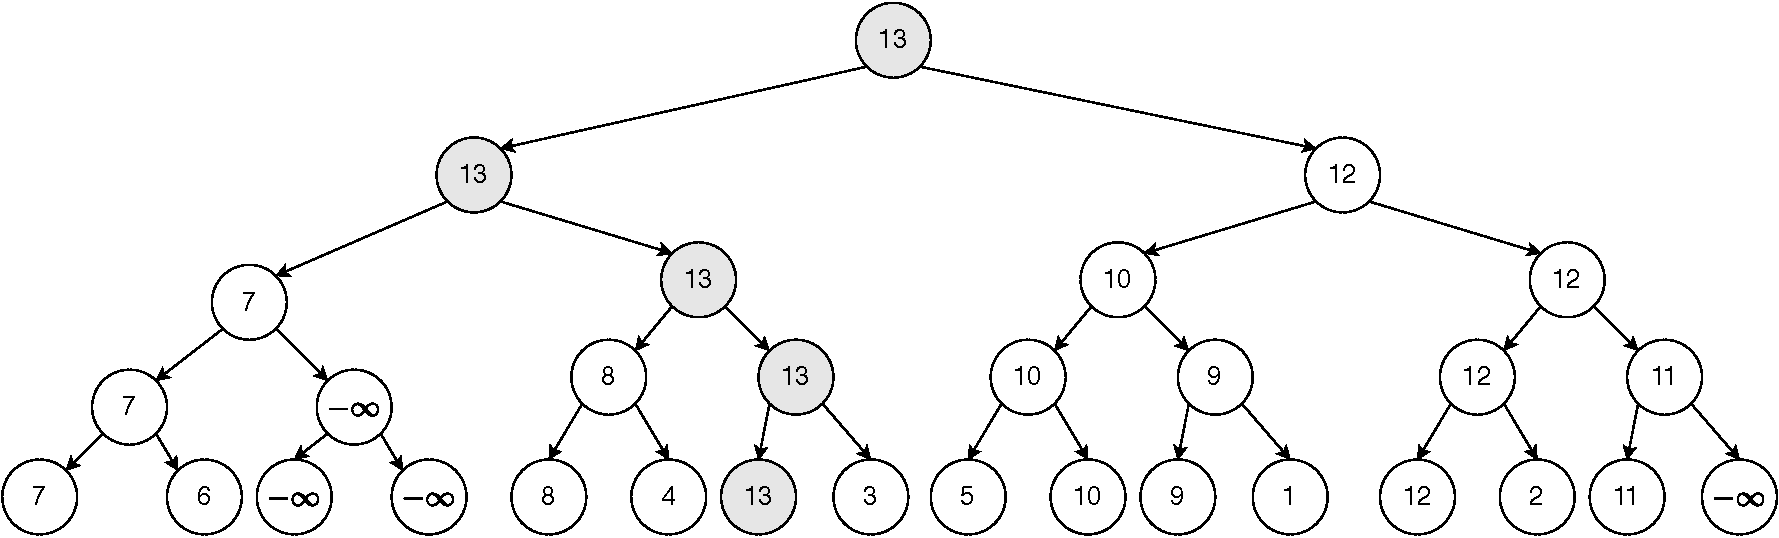
\includegraphics[scale=0.6]{img/tournament-tree-4.ps}}
  \caption{锦标赛树排序的前几步}
  \label{fig:tournament-tree-4}
\end{figure}
\captionsetup[subfigure]{labelformat=parens}

我们可以复用二叉树的定义来表示锦标赛树,为了自底向上回溯,每个节点需要同时指向它的父节点。

\lstset{language=C}
\begin{lstlisting}
struct Node {
    Key key;
    struct Node *left, *right, *parent;
};
\end{lstlisting}

假设待排序的元素有$2^m$个,其中$m$为某个自然数,为了构造锦标赛树,我们先将每个元素放入一个叶子节点中,这样就得到了一组二叉树的列表。每次从列表中取出两棵树,比较它们根节点的值,然后构造一棵较大的二叉树,树根为其中较大的值,参与比较的两棵树分别作为左右子树。重复这一步骤可以得到一组新的树,其中每棵树的高度增加了1。这样一轮过后,新得到的树的数目减半。持续同样的操作最终得到一棵锦标赛树。

\begin{algorithmic}[1]
\Function{Build-Tree}{$A$}
  \State $T \gets \phi$
  \For{each $x \in A$}
    \State $t \gets $ \Call{Create-Node}{}
    \State \Call{Key}{$t$} $\gets x$
    \State \Call{Append}{$T, t$}
  \EndFor
  \While{$|T| > 1$}
    \State $T' \gets \phi$
    \For{every $t_1, t_2 \in$ T}
      \State $t \gets $ \Call{Create-Node}{}
      \State \Call{Key}{$t$} $\gets$ \textproc{Max}(\Call{Key}{$t_1$}, \Call{Key}{$t_2$})
      \State \Call{Left}{$t$} $\gets t_1$
      \State \Call{Right}{$t$} $\gets t_2$
      \State \Call{Parent}{$t_1$} $\gets t$
      \State \Call{Parent}{$t_2$} $\gets t$
      \State \Call{Append}{$T', t$}
    \EndFor
    \State $T \gets T'$
  \EndWhile
  \State \Return $T[1]$
\EndFunction
\end{algorithmic}

设列表$A$的长度为$n$,算法先遍历列表构建树,这一步耗时是线性时间$n$,然后它不断取出一对树进行比较,这一步的时间正比于$n + \frac{n}{2} + \frac{n}{4} + ... + 2 = 2n$。因此整体性能为$O(n)$。

下面的C程序实现了锦标赛树的构造算法。

\lstset{language=C}
\begin{lstlisting}
struct Node* build(const Key* xs, int n) {
    int i;
    struct Node *t, **ts = (struct Node**) malloc(sizeof(struct Node*) * n);
    for (i = 0; i < n; ++i)
        ts[i] = leaf(xs[i]);
    for (; n > 1; n /= 2)
        for (i = 0; i < n; i += 2)
            ts[i/2] = branch(max(ts[i]->key, ts[i+1]->key), ts[i], ts[i+1]);
    t = ts[0];
    free(ts);
    return t;
}
\end{lstlisting}

其中key的类型预先定义好,例如:

\lstset{language=C}
\begin{lstlisting}
typedef int Key;
\end{lstlisting}

函数\texttt{leaf(x)}从值\texttt{x}构建一个叶子节点。节点的左右分支和父节点都为空。函数\texttt{branch(key, left, right)}创建一个分支节点,并且令左右子节点的父指针指向新建的分支节点。我们这里省略了\texttt{leaf}和\texttt{branch}函数的实现细节。读者可以作为练习,尝试实现上述算法。

某些编程环境,例如Python提供了一次迭代两个元素的工具,例如:

\lstset{language=Python}
\begin{lstlisting}
for x, y in zip(*[iter(ts)]*2):
\end{lstlisting}

我们略过这些语言细节,读者可以参考本书附带的代码。

每次取出锦标赛树的根节点后,我们自顶向下将其替换为$-\infty$,然后在通过父指针向上回溯,找出新的最大值。

\begin{algorithmic}[1]
\Function{Extract-Max}{$T$}
  \State $m \gets$ \Call{Key}{$T$}
  \State \Call{Key}{$T$} $\gets -\infty$
  \While{$\lnot$ \Call{Leaf?}{$T$}}  \Comment{自顶向下一轮}
    \If{\textproc{Key}(\Call{Left}{$T$}) $ = m$}
      \State $T \gets$ \Call{Left}{$T$}
    \Else
      \State $T \gets$ \Call{Right}{$T$}
    \EndIf
    \State \Call{Key}{$T$} $\gets -\infty$
  \EndWhile
  \While{\Call{Parent}{$T$} $\neq \phi$} \Comment{自底向上一轮}
    \State $T \gets$ \Call{Parent}{$T$}
    \State \Call{Key}{$T$} $\gets$ \textproc{Max}(\textproc{Key}(\Call{Left}{$T$}), \textproc{Key}(\Call{Right}{$T$}))
  \EndWhile
  \State \Return $m$
\EndFunction
\end{algorithmic}

这一算法返回最大元素,并更改锦标赛树。在真实的编程环境中,由于有限的字长,我们无法使用真正的$-\infty$。通常使用一个相对大的负数,它比锦标赛树中的任何元素都小。例如,若所有的元素都大于-65535,我们可以定义负无穷为:

\lstset{language=C}
\begin{lstlisting}
#define N_INF -65535
\end{lstlisting}

下面的C例子程序实现了这一算法。

\lstset{language=C}
\begin{lstlisting}
Key pop(struct Node* t) {
    Key x = t->key;
    t->key = N_INF;
    while (!isleaf(t)) {
        t = t->left->key == x ? t->left : t->right;
        t->key = N_INF;
    }
    while (t->parent) {
        t = t->parent;
        t->key = max(t->left->key, t->right->key);
    }
    return x;
}
\end{lstlisting}

\textproc{Extract-Max}的行为和某些数据结构的弹出操作非常类似。例如队列和堆,因此我们在上述代码中将其命名为\texttt{pop}。

\textproc{Extract-Max}上下处理树两遍,首先自顶向下一遍,接着自底向上沿着“冠军之路”一遍。由于锦标赛树是平衡的,路径的长度,也就是树的高度为$O(\lg n)$,其中$n$是待排序元素的数目(也就是叶子节点的数目)。因此算法的性能为$O(\lg n)$。

为了实现锦标赛淘汰排序算法,我们先从待排序元素构造一棵锦标赛树,然后不断取出最大值。如果我们希望按照单调递增的顺序排序,我们将第一个取出的元素放在最右侧,然后将后继取出的元素依次向左侧放;否则,如果是降序排序,我们不断将取出的元素追加到结果的末尾。下面的算法按照升序进行排序。

\begin{algorithmic}[1]
\Procedure{Sort}{$A$}
  \State $T \gets$ \Call{Build-Tree}{$A$}
  \For{$i \gets |A|$ down to $1$}
    \State $A[i] \gets$ \Call{Extract-Max}{$T$}
  \EndFor
\EndProcedure
\end{algorithmic}

下面的C例子程序实现了上述排序算法。

\lstset{language=C}
\begin{lstlisting}
void tsort(Key* xs, int n) {
    struct Node* t = build(xs, n);
    while(n)
        xs[--n] = pop(t);
    release(t);
}
\end{lstlisting}

算法首先使用$O(n)$时间构建一棵锦标赛树,然后执行$n$次弹出操作,逐一从树中取出剩余元素的最大值。因为每次弹出操作的性能为$O(\lg n)$,所以锦标赛淘汰排序算法的总体性能为$O(n \lg n)$。

\subsubsection{锦标赛淘汰法的细节改进}
\index{锦标赛淘汰法!显式无穷}

锦标赛淘汰法也可以用纯函数式的方式实现。我们会看到弹出操作中的两遍处理过程(第一遍自顶向下将冠军替换为$-\infty$;第二遍自底向上查找新的冠军)可以通过递归合并起来。于是不再需要存储父节点的引用。我们可以复用函数式的二叉树定义,如下面的例子Haskell代码所示:

\lstset{language=Haskell}
\begin{lstlisting}[style=Haskell]
data Tr a = Empty | Br (Tr a) a (Tr a)
\end{lstlisting}

一棵二叉树或者为空,或者为一个分支节点,包含一个key和左右子树。每棵子树都是一棵二叉树。

此前,我们使用一个较大的负整数来表示$-\infty$。但是这个方法是临时性的,有诸多不便。某些编程环境支持代数类型,这样就可以明确定义负无穷。例如下面的Haskell程序建立了无穷的定义\footnote{如果希望直接使用默认的\texttt{Ord}来比较大小,则需要按照负无穷、普通数字和正无穷的顺序来声明。当然,也可以将我们的类型声明为\texttt{Ord}的一个instance,然后给出大小比较的规则。这些是语言特有的性质,超出了本书的范围。读者可以参考其他Haskell资料}.。

\lstset{language=Haskell}
\begin{lstlisting}[style=Haskell]
data Infinite a = NegInf | Only a | Inf deriving (Eq, Ord)
\end{lstlisting}

接下来的部分,我们使用$min()$函数来决定比赛的胜者,相应的锦标赛树选择最小的元素作为冠军。

记函数$key(T)$返回树$T$根节点的key。函数$wrap(x)$将元素$x$装入一个叶子节点。函数$tree(l, k, r)$构造一个分支节点。其中$k$是key,$l$和$r$分别是左右分支。

在淘汰过程中,我们比较两棵树,选择较小的key作为新节点的key,进行比较的两棵树作为左右子树。

\be
branch(T_1, T_2) = tree(T_1, min(key(T_1), key(T_2)), T_2)
\ee

对应的Haskell例子代码为:

\lstset{language=Haskell}
\begin{lstlisting}[style=Haskell]
branch t1 t2 = Br t1 (min (key t1) (key t2)) t2
\end{lstlisting}

此前的锦标赛排序算法有一个限制。它要求待排序的元素个数必须是$2^m$,否则我们无法构造一棵完全二叉树。现在考虑如何克服这一问题。每次我们都选出两棵树,比较并且选择较大的。如果树的总数目为偶数,我们总能不断选出两棵。在真正的足球比赛中,如果某支球队因故缺席了比赛(例如航班延误),则会有一支球队没有对手。可以规定这支球队为胜者,直接进入接下来的比赛。我们完全可以使用类似的方法。

首先将每个元素都装入叶子节点,然后开始构造锦标赛树。

\be
build(L) = build'(\{wrap(x) | x \in L\})
\ee

函数$build'(\mathbb{T})$中,如果列表$\mathbb{T}$中仅有一棵树,则此树就是最终结果。否则,它将每两棵树分成一组,然后决定胜者。如果有奇数棵树,就规定最后一棵树为胜者,可以进入下一轮比赛。然后我们递归调用这一构造算法。

\be
build'(\mathbb{T}) = \left \{
  \begin{array}
  {r@{\quad:\quad}l}
  \mathbb{T} & |\mathbb{T}| \leq 1 \\
  build'(pair(\mathbb{T})) & otherwise
  \end{array}
\right.
\ee

这一算法还能处理另外一种特殊情况:如果待排序的列表为空,则结果也为空。

如果列表中至少有两棵树,记$\mathbb{T} = \{ T_1, T_2, ...\}$,而$\mathbb{T}'$表示除最初两棵树外的剩余树。函数$pair(\mathbb{T})$定义如下:

\be
pair(\mathbb{T}) = \left \{
  \begin{array}
  {r@{\quad:\quad}l}
  \{ branch(T_1, T_2) \} \cup pair(\mathbb{T}') & |\mathbb{T}| \geq 2 \\
  \mathbb{T} & otherwise
  \end{array}
\right.
\ee

下面的Haskell例子代码给出了构造锦标赛树的完整程序。

\lstset{language=Haskell}
\begin{lstlisting}[style=Haskell]
fromList :: (Ord a) => [a] -> Tr (Infinite a)
fromList = build . (map wrap) where
  build [] = Empty
  build [t] = t
  build ts = build $ pair ts
  pair (t1:t2:ts) = (branch t1 t2):pair ts
  pair ts = ts
\end{lstlisting} %$

为了从锦标赛树中取得冠军(最小元素),我们检查左右子树,看哪一棵子树的key和根节点的key相等。然后递归地从子树中取出冠军直到到达叶子节点。记$T$的左子树为$L$,右子树为$R$,$K$为key,弹出算法可以定义如下:

\be
pop(T) =  \left \{
  \begin{array}
  {r@{\quad:\quad}l}
  tree(\phi, \infty, \phi) & L = \phi \land R = \phi \\
  tree(L', min(key(L'), key(R)), R) & K = key(L), L' = pop(L) \\
  tree(L, min(key(L), key(R')), R') & K = key(R), R' = pop(R)
  \end{array}
\right.
\ee

下面的Haskell例子代码实现了弹出算法。

\lstset{language=Haskell}
\begin{lstlisting}[style=Haskell]
pop (Br Empty _ Empty) = Br Empty Inf Empty
pop (Br l k r) | k == key l = let l' = pop l in Br l' (min (key l') (key r)) r
               | k == key r = let r' = pop r in Br l (min (key l) (key r')) r'
\end{lstlisting}

注意这一算法仅仅将冠军元素删除而没有返回,因此有必要定义另外一个函数从根节点提取冠军元素。

\be
top(T) = key(T)
\ee

使用这些定义好的函数,锦标赛淘汰排序法可以形式化为下面的等式:

\be
sort(L) = sort'(build(L))
\ee

其中$sort'(T)$不断从锦标赛树中弹出最小的元素:

\be
sort'(T) = \left \{
  \begin{array}
  {r@{\quad:\quad}l}
  \phi & T = \phi \lor key(T) = \infty \\
  \{ top(T) \} \cup sort'(pop(T)) & otherwise
  \end{array}
\right.
\label{eq:tsort}
\ee

下面的Haskell例子程序实现了完整的锦标赛淘汰排序算法。

\lstset{language=Haskell}
\begin{lstlisting}[style=Haskell]
top = only . key

tsort :: (Ord a) => [a] -> [a]
tsort = sort' . fromList where
    sort' Empty = []
    sort' (Br _ Inf _) = []
    sort' t = (top t) : (sort' $ pop t)
\end{lstlisting} %$

其中用以支持无穷类型的辅助函数\texttt{only}、\texttt{key}和\texttt{wrap}定义如下:

\lstset{language=Haskell}
\begin{lstlisting}[style=Haskell]
only (Only x) = x
key (Br _ k _ ) = k
wrap x = Br Empty (Only x) Empty
\end{lstlisting}

\begin{Exercise}
  \begin{itemize}
    \item 实现命令式锦标赛淘汰法中的辅助函数\texttt{leaf()}、\texttt{branch}、\texttt{max()}、\texttt{isleaf()}和\texttt{release()}。
    \item 在一门支持垃圾回收(GC)的语言中实现命令式的锦标赛淘汰法排序程序。
    \item 为什么我们的锦标赛树淘汰法排序程序可以处理重复元素(元素的值相等)?如果相等元素的顺序经过排序后保持不变,我们称之为稳定排序。锦标赛树淘汰法排序是稳定排序么?
    \item 设计一个命令式的锦标赛淘汰排序算法,满足下面的条件:
      \begin{itemize}
        \item 可以处理任意数目的元素;
        \item 不使用硬编码(hard code)的大负数,可以处理任意值的元素。
      \end{itemize}
    \item 比较锦标赛树淘汰算法和二叉搜索树排序算法,分析它们的时间和空间效率。
    \item 比较堆排序算法和二叉搜索树排序算法,分析它们的时间和空间效率。
  \end{itemize}
\end{Exercise}

\subsection{使用堆排序进行最后的改进}

通过使用锦标赛树淘汰法,我们将基于选择的排序算法性能提高到$O(n \lg n)$。这已经达到了基于比较的排序算法的上限\cite{TAOCP}。但是,这里仍然有提高的空间。排序完成后,锦标赛树的所有节点都变成了负无穷,这棵完全二叉树不再含有任何有用的信息,但它却占据了很大空间。有没有办法在弹出后释放节点呢?

另外我们可以观察到,如果待排序的元素有$n$个,我们实际上使用了$2n$个节点。其中有$n$个叶子和$n$个分支。有没有办法能节约一半空间呢?

如果我们认为根节点的key为无穷,则树为空,那么上一节最后给出的公式\ref{eq:tsort}就可以进一步概括为更加通用的形式:

\be
sort'(T) = \left \{
  \begin{array}
  {r@{\quad:\quad}l}
  \phi & T = \phi\\
  \{ top(T) \} \cup sort'(pop(T)) & otherwise
  \end{array}
\right.
\ee

这和我们在上一章堆排序给出的公式完全一样。堆总是在顶部保存最小(或最大)值,并且提供了快速的弹出操作。使用数组的binary堆实际上将树结构“编码”成数组的索引,因此除了$n$个单元外,无需任何额外的空间。函数式的堆,如左偏堆和splay堆也只需要$n$个节点。我们将在下一章介绍更多种类的堆,它们在许多情况下都有很好的性能。

\section{小结}

本章我们介绍了选择排序的进化过程。选择排序简单、直观,经常被用来教授编程中的多重循环。它的结构虽然简单,但是性能却是平方级别的。本章中,我们看到,选择排序不仅可以通过细微调整加以改进,而且还可以通过改变底层的数据结构,进化到锦标赛淘汰排序和堆排序,从而在本质上得到性能的提升。

\ifx\wholebook\relax\else
\begin{thebibliography}{99}

\bibitem{TAOCP}
Donald E. Knuth. ``The Art of Computer Programming, Volume 3: Sorting and Searching (2nd Edition)''. Addison-Wesley Professional; 2 edition (May 4, 1998) ISBN-10: 0201896850 ISBN-13: 978-0201896855

\bibitem{CLRS}
Thomas H. Cormen, Charles E. Leiserson, Ronald L. Rivest and Clifford Stein.
``Introduction to Algorithms, Second Edition''. ISBN:0262032937. The MIT Press. 2001 (《算法导论》中文版)

\bibitem{wiki-sweak-order}
Wikipedia. ``Strict weak order''. \url{https://en.wikipedia.org/wiki/Strict_weak_order}

\bibitem{wiki-wc}
Wikipedia. ``FIFA world cup''. \url{https://en.wikipedia.org/wiki/FIFA_World_Cup}

\end{thebibliography}

\end{document}
\fi
